\section{Proposal: merge L1 and L2 farm}

\begin{frame}{Infrastructure planned so far}{}
	\begin{center} 
		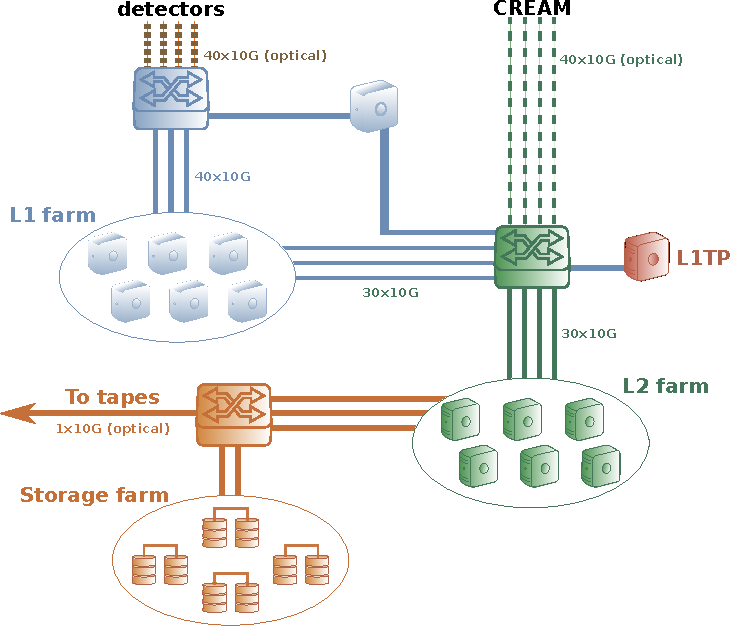
\includegraphics[width=8cm]{whole-farm-orig}
	\end{center} 
\end{frame}

\begin{frame}{Logical data flow so far}{Waste of resources?!}
	\begin{center} 
		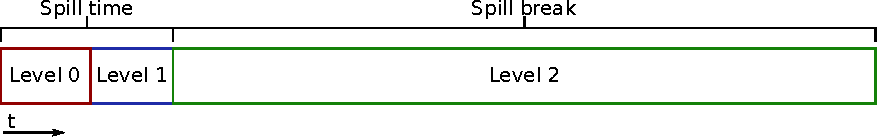
\includegraphics[width=\textwidth]{spilltime}
	\end{center} 
		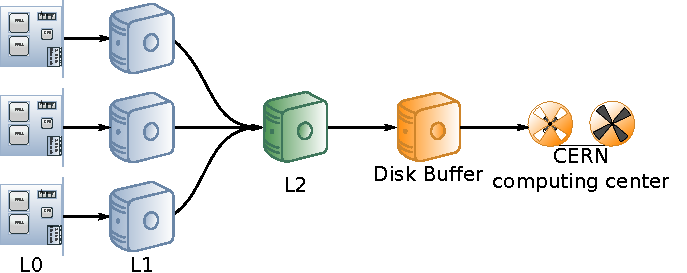
\includegraphics[height=4cm]{dataflow-logical}
\end{frame}

\begin{frame}{Merge L1 and L2}{More efficient load distribution}
	\begin{center} 
		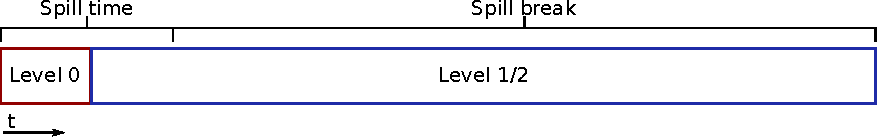
\includegraphics[width=\textwidth]{spilltime-l12merged}
	\end{center} 
		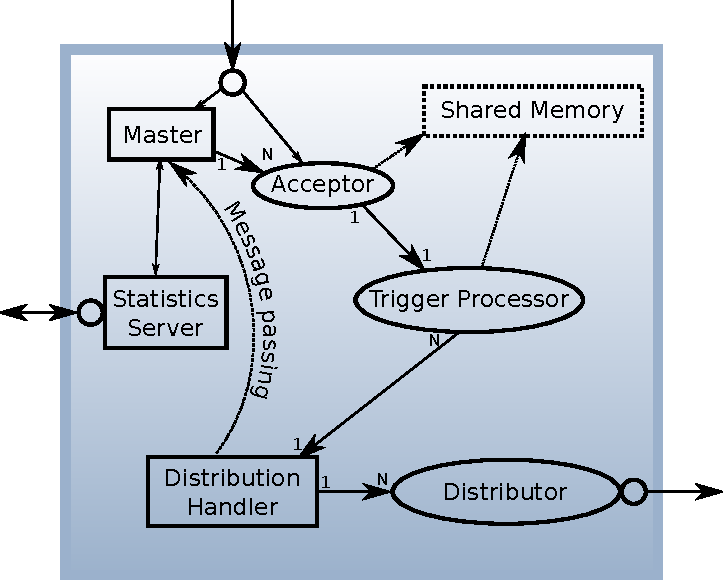
\includegraphics[height=4cm]{dataflow}
\end{frame}

\begin{frame}{Data flow and trigger decision}{}
	\begin{center} 
		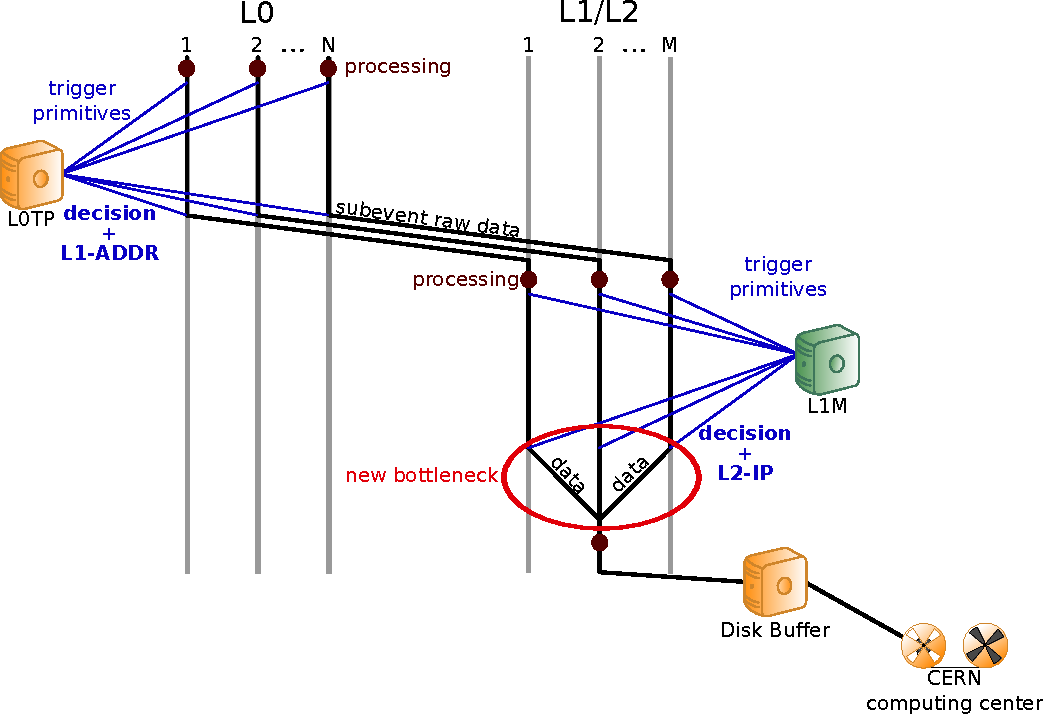
\includegraphics[width=\textwidth]{dataflow-trigger-decision}
	\end{center} 
\end{frame}

\begin{frame}{Problems merging L1 and L2}{}
\begin{alertblock}{Now you have two incoming data flows for one Cluster}
	Each PC now has to process L1 and L2 and you need a good load balancing so that
	L1 still can process the L0 data quick enough.
\end{alertblock}
		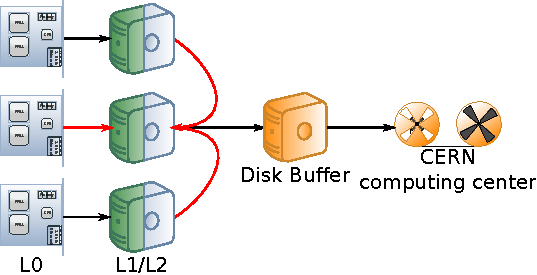
\includegraphics[height=4cm]{dataflow-alert}
\end{frame}

\begin{frame}{Caching solves bottleneck and disposes additional switch}{}
		\begin{block}{To reduce network
	traffic: Don't start EB/L2 before L1 finished}
		\begin{itemize}
			\item Need to store $\approx100kHz*5kB=500MBps$ data in memory during
			spill \tiny(see table 61 in TDR) \normalsize{}! That's negligible.
		\end{itemize}
	\end{block}
	
	\begin{ergo}
		By holding data in cache until L1 has finished you need only one switch as you
		can use it for L0-L1 and L1-L2 transmission at separate times. Than the merged
		cluster also doesn't need to be bigger than the old L1 or L2 cluster ($\approx
		50 \%$ less PCs)
	\end{ergo}
\end{frame}

\begin{frame}{Overview with L1 and L2 separated}{}
	\begin{center} 
		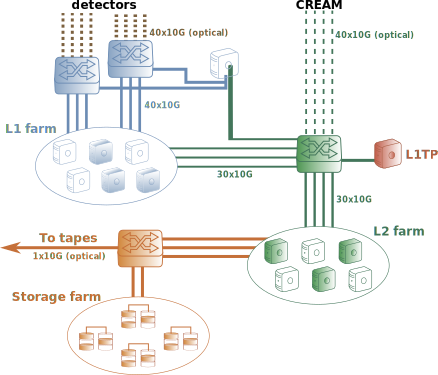
\includegraphics[width=8cm]{whole-farm}
	\end{center} 
\end{frame}

\begin{frame}{Overview with L1 and L2 merged}{Need one huge core switch}
	\begin{center} 
		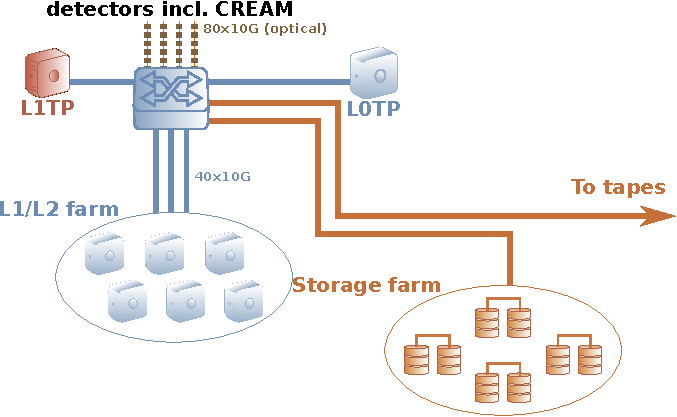
\includegraphics[width=0.8\textwidth]{whole-farm-l12merged}
	\end{center} 
\end{frame}

\begin{frame}{Proposals by www.SEiCOM-muc.de}{}
	\begin{columns}
	 	\column{.5\textwidth}
			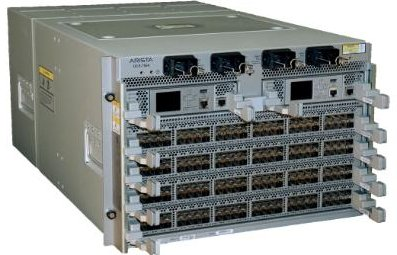
\includegraphics[width=2cm]{arista-7504}
			\begin{block}{Arista 7504}
				\begin{itemize}
				  \item Chassis + Supervisor: \\44,400€
				  \item 3*48-port linecards: \\67,638€
				  \item Redundant supervisor: \\6,829€
				  \item 60*SFP+ SR (up to 220m): \\21,780€
				\end{itemize}
			\end{block}
			\center{\textbf{141 k€}}
						
	    \column{.5\textwidth}
	    	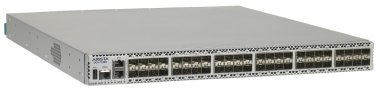
\includegraphics[width=2cm]{arista-7148s}
	    	\begin{block}{Arista 7148S}
				\begin{itemize}
				  \item 3 *48 port switch: \\44,400€
				  \item 3*48-port Linecards: \\67,638€
				  \item 60*SFP+ SR (up to 220m): \\21,780€
				  \item Redundant power supply included
				\end{itemize}
			\end{block}
			\center{\textbf{66 k€}}
	\end{columns}
\end{frame}






\section{Proposal for a farm framework}
\begin{frame}{Online farm framework}{}
	\begin{center}
	  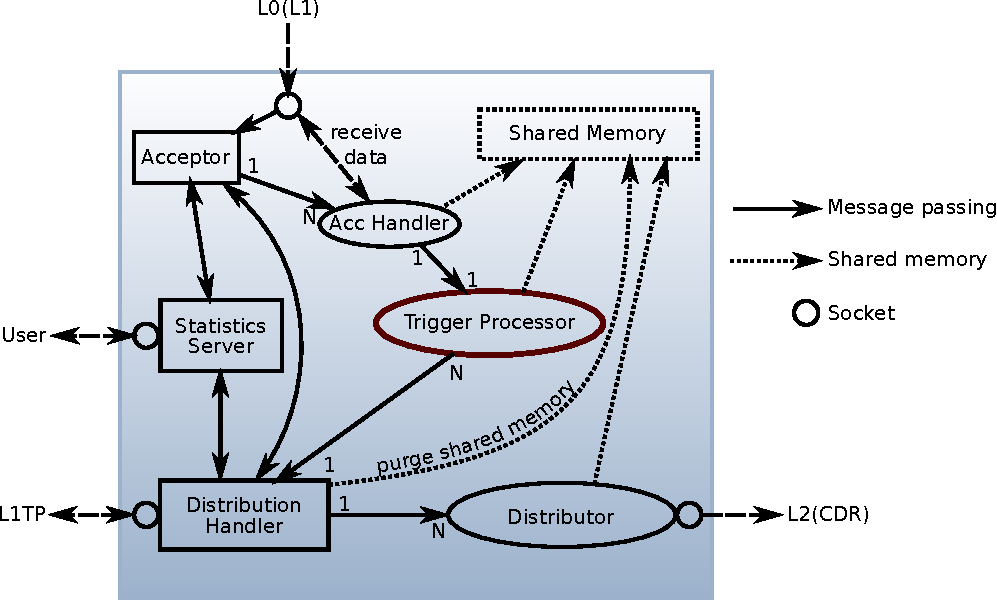
\includegraphics[width=0.97\textwidth]{processes}
	\end{center}
\end{frame}

\begin{frame}{TriggerProcessor Class}{}
	\begin{exampleblock}{Parent Class designed by me, inherited and implemented by the
	subdetector groups}
	TriggerPrimitive processData(char* data) const;
	\end{exampleblock}
	
	\begin{block}{What will TriggerPrimitive Class look like?}
		std::size\_t getEventID() const; \\
		bool disposeEvent() const; \\
		char* getReconstructedData() const;
	\end{block}
	
\end{frame}